\begin{frame}{selected HTTP methods}
\small
\begin{tabular}{lllll}
method & purpose & request body? & respones body? & `safe' \\
GET & retrieve resource & never & usually & yes \\
HEAD & retrieve resource headers& never & never & yes \\
POST & provide data & always & usually & no \\
PUT & set contents of resource & always & maybe & no \\
DELETE & delete resource & never & maybe & no \\
OPTIONS & get info about server & maybe & maybe & no \\
\end{tabular}
\end{frame}

\begin{frame}{safety}
    \begin{itemize}
    \item GET, HEAD = `safe' methods
    \item okay for clients to repeat, send unprompted
        \begin{itemize}
        \item `prefetch' resources
        \item redo when user presses back button unprompted
        \end{itemize}
    \item other methods: that's not okay!
    \end{itemize}
\begin{center}
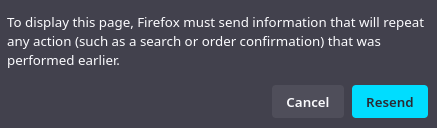
\includegraphics[width=0.7\textwidth]{../http/ff-resend-warning}
\end{center}
\end{frame}

